\documentclass[12pt]{article}
%% arXiv paper template by Flip Tanedo
%% last updated: Dec 2016


%%%%%%%%%%%%%%%%%%%%%%%%%%%%%
%%%  THE USUAL PACKAGES  %%%%
%%%%%%%%%%%%%%%%%%%%%%%%%%%%%

\usepackage{amsmath}
\usepackage{amssymb}
\usepackage{amsfonts}
\usepackage{graphicx}
\usepackage{xcolor}
\usepackage{nopageno}
\usepackage{enumerate}
\usepackage{parskip}

%%%%%%%%%%%%%%%%%%%%%%%%%%%%%%%%%
%%%  UNUSUAL PACKAGES        %%%%
%%%  Uncomment as necessary. %%%%
%%%%%%%%%%%%%%%%%%%%%%%%%%%%%%%%%

%% MATH AND PHYSICS SYMBOLS
%% ------------------------
%\usepackage{slashed}       % \slashed{k}
%\usepackage{mathrsfs}      % Weinberg-esque letters
%\usepackage{youngtab}	    % Young Tableaux
%\usepackage{pifont}        % check marks
\usepackage{bbm}           % \mathbbm{1} incomp. w/ XeLaTeX 
%\usepackage[normalem]{ulem} % for \sout


%% CONTENT FORMAT AND DESIGN (below for general formatting)
%% --------------------------------------------------------
\usepackage{lipsum}        % block of text (formatting test)
%\usepackage{color}         % \color{...}, colored text
%\usepackage{framed}        % boxed remarks
%\usepackage{subcaption}    % subfigures; subfig depreciated
%\usepackage{paralist}      % compactitem
%\usepackage{appendix}      % subappendices
%\usepackage{cite}          % group cites (conflict: collref)
%\usepackage{tocloft}       % Table of Contents	

%% TABLES IN LaTeX
%% ---------------
%\usepackage{booktabs}      % professional tables
%\usepackage{nicefrac}      % fractions in tables,
%\usepackage{multirow}      % multirow elements in a table
%\usepackage{arydshln} 	    % dashed lines in arrays

%% Other Packages and Notes
%% ------------------------
%\usepackage[font=small]{caption} % caption font is small



\renewcommand{\thesection}{}
\renewcommand{\thesubsection}{\arabic{subsection}}

%%%%%%%%%%%%%%%%%%%%%%%%%%%%%%%%%%%%%%%%%%%%%%%
%%%  PAGE FORMATTING and (RE)NEW COMMANDS  %%%%
%%%%%%%%%%%%%%%%%%%%%%%%%%%%%%%%%%%%%%%%%%%%%%%

\usepackage[margin=2cm]{geometry}   % reasonable margins

\graphicspath{{figures/}}	        % set directory for figures

% for capitalized things
\newcommand{\acro}[1]{\textsc{\MakeLowercase{#1}}}    

\numberwithin{equation}{subsection}    % set equation numbering
\renewcommand{\tilde}{\widetilde}   % tilde over characters
\renewcommand{\vec}[1]{\mathbf{#1}} % vectors are boldface

\newcommand{\dbar}{d\mkern-6mu\mathchar'26}    % for d/2pi
\newcommand{\ket}[1]{\left|#1\right\rangle}    % <#1|
\newcommand{\bra}[1]{\left\langle#1\right|}    % |#1>
\newcommand{\Xmark}{\text{\sffamily X}}        % cross out


\let\olditemize\itemize
\renewcommand{\itemize}{
  \olditemize
  \setlength{\itemsep}{1pt}
  \setlength{\parskip}{0pt}
  \setlength{\parsep}{0pt}
}


% Commands for temporary comments
\newcommand{\comment}[2]{\textcolor{red}{[\textbf{#1} #2]}}
\newcommand{\flip}[1]{{\color{red} [\textbf{Flip}: {#1}]}}
\newcommand{\email}[1]{\texttt{\href{mailto:#1}{#1}}}

\newenvironment{institutions}[1][2em]{\begin{list}{}{\setlength\leftmargin{#1}\setlength\rightmargin{#1}}\item[]}{\end{list}}


\usepackage{fancyhdr}		% to put preprint number



%%%%%%%%%%%%%%%%%%%
%%%  HYPERREF  %%%%
%%%%%%%%%%%%%%%%%%%

%% This package has to be at the end; can lead to conflicts
\usepackage{microtype}
\usepackage[
	colorlinks=true,
	citecolor=black,
	linkcolor=black,
	urlcolor=green!50!black,
	hypertexnames=false]{hyperref}



%%%%%%%%%%%%%%%%%%%%%
%%%  TITLE DATA  %%%%
%%%%%%%%%%%%%%%%%%%%%

\begin{document}


\begin{center}

    {\Large \textsc{Homework 3b:} 
    \textbf{Complex Analysis}}
    
\end{center}

\vskip .4cm

\noindent
\begin{tabular*}{\textwidth}{rlcrll}
	\textsc{Course:}& Physics 231, \emph{Methods of Theoretical Physics} (2018)
	&
%	\hspace{1.2cm}
	&
	\\
	\textsc{Instructor:}& Professor Flip Tanedo (\email{flip.tanedo@ucr.edu})
	&
	%\hfill
	&
	& 
	\\
	\textsc{Due by:}& Mon, November 12
	&
	%\hfill
	&
	%	
\end{tabular*}



\subsection{Practice with complex integration}

\textbf{Remark}: This was originally posed in Homework 2B problem 3. If you already did it, please note ``already submitted.'' If you did not complete it---for example, because we didn't get to the material in our discussions---then please complete them as part of this homework.

% Boas 14.3.1

\subsubsection{This is not a closed loop}

The goal of this problem is to review line integrals in a 2D space. Perform the integral
\begin{align}
	\int_i^{1+i} dz \; z \,
\end{align}
with respect to the path that connects $z=i$ and $z=i+1$ by a straight line segment. This is \emph{not} a closed loop, there's no magic formula for this. Just parameterize the path by writing $z$ as a function of a real parameter. Then write out $dz$ in terms of the parameter. Do the integral.

\subsubsection{Contour integrals}

Calculate the following integrals using the residue theorem:
\begin{enumerate}[(a)]
	\item $\displaystyle \int_{0}^\infty \frac{x^2}{x^4 + 16} dx$ % Boas ch 7 probs
	\item $\displaystyle \int_{-\infty}^\infty \frac{\sin x}{x^2 + 4x + 5}dx$ % Boas ch 7 probs
	\item $\displaystyle \int_{0}^\infty \frac{1}{x^6+1}dx$ using a contour including the real line and a large semicircle in the complex plane % Appel ch 4 probs
	\item $\displaystyle \int_{0}^\infty \frac{1}{x^6+1}dx$ using a contour that encloses the `pizza slice' wedge between $\theta = 0$ and $\theta = \pi/3$. 
\end{enumerate}

\textsc{Hint}: for (d), the line integral along the diagonal is proportional to the integral you want. % Appel ch 4 probs






\subsection{How to find Residues}

This problem is based on Boas (page 599) and Appel (section 4.5d).
%
We saw that a \textbf{meromorphic} (analytic up to poles) function has a Laurent series expansion about a point $z_0$,
\begin{align}
f(z) &= \sum_{n=-\infty}^{\infty} a_n (z-z_0)^n
	\ .
\end{align}
The $a_{-1}$ term has special significance and is known as the \textbf{residue} of $f$ at $z_0$, $\text{Res}(f,z_0)$. When we have an explicit Laurent expansion about $z_0$, identifying the residue is a matter of reading off the $(z-z_0)^{-1}$ coefficient. Alternately, when $z_0$ is a simple pole the function can be written as
\begin{align}
	f(z) = \frac{F(z)}{(z-z_0)} \ ,
\end{align}
where $F(z)$ is analytic at $z_0$. In this case, the residue is $\text{Res}(f,z_0) = F(z_0)$. This leads to the sometimes useful guide: If $f(z_0)$ is not finite but $(z-z_0)\, f(z)$ is finite, then
	\begin{align}
		\text{Res}(f,z_0) &=  \lim_{z\to z_0} (z-z_0)\, f(z) \ .
	\end{align}
What do we do if $(z-z_0)\, f(z)$ is \emph{not} finite? For example, what if both $a_{-1}$ and $a_{-2}$ were non-zero? How does determine the residue ($a_1$) in such a case? Explain why the following algorithm works: Find the positive integer $m$ such that $F_m(z)=(z-z_0)^m f(z)$ is finite at $z=z_0$, then the residue is
\begin{align}
	\text{Res}(f,z_0) = \left.\frac{1}{(m-1)!} \frac{d^{m-1}}{dz^{m-1}} F_m(z)\right|_{z=z_0} \ .
\end{align}






\subsection{A Fourier transform refresher}
%https://physics.stackexchange.com/questions/308234/fourier-transform-standard-practice-for-physics/308252

Fourier transforms are annoying because there are a few choices that one has to make to establish conventions. The convention that we will use is: % consistent with Peskin
\begin{align}
	f(x) &= \int \frac{dk}{2\pi} e^{-ikx}\, \tilde f(k)
	&
	\tilde f(k) &= \int dx \, e^{ikx}\, f(x) \ .
\end{align}
In this convention, the $(2\pi)$ comes with the $dk$, so I will often write $\dbar k = dk/(2\pi)$.

\subsubsection{Fourier decomposition of $\delta(x)$}

What is the Fourier transform of $\delta(x)$? In other words, find $\tilde \delta(k)$ in
\begin{align}
	\delta(x) = \int \dbar k \, e^{ikx}\, \tilde\delta(k) \ .
\end{align}
What about $\delta(x-x_0)$?

\subsubsection{Other conventions}
%https://physics.stackexchange.com/questions/308234/fourier-transform-standard-practice-for-physics

A general convention for the Fourier transform is:
\begin{align}
	f(x) &= |B|^{1/2}
	\int \frac{dk}{\sqrt{(2\pi)^{1+A}}} \, e^{-iBkx} \tilde f(k)
	&
	\tilde f(k) &= |B|^{1/2}
	\int \frac{dx}{\sqrt{(2\pi)^{1-A}}} \, e^{iBkx} f(x) \ .
\end{align}
Our conventions correspond to $B=1$ and $A=1$. Show that in this general form, the inverse Fourier transform of a Fourier transform is simply the original function. 

\subsubsection{Higher dimensions}

In two Euclidean dimensions, the Fourier transform is
\begin{align}
	f(x, y) = \int\frac{dx}{2\pi} \int\frac{dy}{2\pi} \, e^{-ik_xx} e^{-ik_yy} \tilde f(k_x, k_y) \ .
\end{align}
This can be rewritten in terms of a position 2-vector\footnote{Mathematicians laugh at us when we say `position vector.'} $\vec{x}$ and corresponding momentum 2-vector $\vec{k}$ \ , 
\begin{align}
	f(\vec x) = \int\frac{d^2\vec x}{(2\pi)^2}  \, e^{-i\vec k\cdot \vec y} \tilde f(\vec k) \ .
\end{align}
Observe that the exponential is built out of the rotationally-invariant scalar quantity, $\vec k\cdot \vec y$. 
%
When we deal with \emph{partial} differential equations, we'll need to Fourier transform in multiple dimensions. Sometimes we'll have to Fourier transform in both time and space. It is conventional to choose signs so that we may write this as 
\begin{align}
	f(x, t) = \int\frac{dx}{2\pi} \int\frac{dt}{2\pi} \, e^{+ikx} e^{-i\omega t} \tilde f(k, \omega) \ .
\end{align}
Briefly comment why this is a good idea from two points of view:
\begin{enumerate}
	\item The idea that we are expanding about a basis of traveling plane waves. 
	\item Lorentz invariance, in case we want our expressions to respect special relativity.
\end{enumerate}

\subsection{Integral representation of the step function}
% Cahill Problem 5.32

[\textsc{Cahill}, Problem 5.32] 
The step function is defined by $\Theta(x) = 0$ for $x<0$ and $\Theta(x) = 1$ for $x>0$. Show that this is equivalent to
\begin{align}
	\Theta(x) = \frac{1}{2\pi i}\int_{-\infty}^\infty \frac{e^{ixz}}{z-i\varepsilon} dz \ .
\end{align}

\textsc{Hint}: What does the $-i\epsilon$ mean? Compare this to the advanced and retarded Green's functions that we explored in Lecture 15. 


\subsection{Evaluating an NSF GRFP proposal}

There is a sample NSF Graduate Research Fellowship proposal posted on this course's \texttt{iLearn} page under Course Materials. The proposal is from a recent Caltech graduate student who won the fellowship and has shared these materials to help other graduate students who are applying in the future. Please read the two essays (personal statement and research statement). Please answer the following:
\begin{enumerate}
	\item What did you like about the research statement? What did you find difficult to read?
	\item What did you like about the personal statement? What did you find difficult to read?
	\item Think about the visual format of the document. Given that an NSF reviewer reads dozens of these at a time, how did the formatting help/hurt the statements? Consider the spacing, use of \textbf{bold} text, sectioning, etc.
	\item The research statement is tricky because you have to show competency in a field that you are just entering. Comment on how much progress the author has made on the proposed study at the time that the proposal was written. What kind of tasks have already been complete (e.g. discussions with faculty, literature reviews, ...) and what remains to be done (e.g. has a data analysis pipeline already been developed?). 
	\item Comment on how the tone and purpose of the personal statement in contrast to the research statement. What parts of the personal narrative did the author think it was important to highlight for the reviewer?
\end{enumerate}





\section{Extra Credit}

These problems are not graded and are for your edification. You are strongly encouraged to explore and discuss these topics, especially if they are in a field of interest to you.


\subsection{Laurent Theorem}

We shall prove the Laurent Theorem for the expansion about $z_0$ of a function $f(z)$ in a region where it is meromorphic:
\begin{align}
f(z) &= \sum_{n=-\infty}^{\infty} a_n (z-z_0)^n
&
a_n &= \frac{1}{2\pi i} \oint_C \frac{f(z)}{(z-z_0)} dz \ ,
\end{align}
where $C$ is a contour that loops once counter-clockwise around $z_0$.

Consider the contour below (image from Cahill, \emph{Physical Mathematics}), enclosing an annular region that includes the point $z$ without any poles (asterisks).
\begin{center}
% Image from Cahill, Fig 5.5
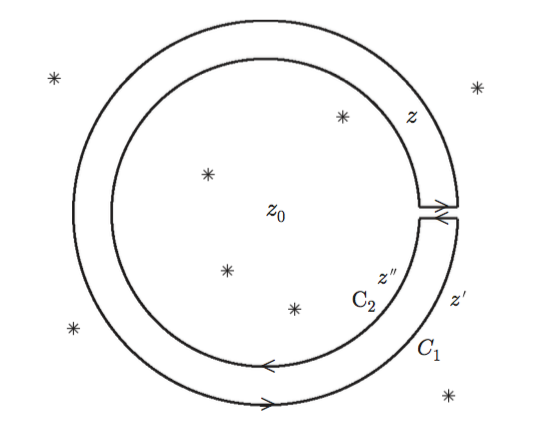
\includegraphics[width=.5\textwidth]{P231_2018_HW3a_fig3}
\end{center}
Both the outer and inner contours, $C_1$ and $C_2$, encircle $z_0$. Use the \textbf{Cauchy theorem},
\begin{align}
	f(z) = \frac{1}{2\pi i} \oint_{C} \frac{f(w)}{w-z_0} dw \ ,
	\label{eq:laurent}
\end{align}
where $C$ encloses a region in which $f(z)$ is \emph{analytic}. Taking $C = C_1 - C_2$, the contour shown above, one has
\begin{align}
	f(z) = 
	\frac{1}{2\pi i} \oint_{C_1} \frac{f(z')}{z'-z} dz'
	-
	\frac{1}{2\pi i} \oint_{C_2} \frac{f(z'')}{z''-z} dz'' \ .
	\label{eq:laurent:int}
\end{align}
Consider the following quantities:
\begin{align}
	r(z') &= \frac{z-z_0}{z'-z_0}
	&
	R(z'') &= \frac{z - z_0}{z''-z_0} \ .
\end{align}
Note that $|r(z)| < 1$ and $|1/R(z)| < 1$. Write (\ref{eq:laurent:int}) as
\begin{align}
	f(z) = 
	\frac{1}{2\pi i} \oint_{C_1} \frac{f(z')}{(z'-z_0)\left[1-r(z')\right]} dz'
	-
	\frac{1}{2\pi i} \oint_{C_2} \frac{f(z'')}{(z-z_0)\left[1-1/R(z'')\right]} dz'' \ .
\end{align}
Use the series expansion
\begin{align}
	\frac{1}{1-s} = \sum_{n=0}^\infty s^n \ ,
\end{align}
for $|s|<1$. Argue that we may now deform $C_1$ and $C_2$ to an intermediate contour $C$. Show that the result of all this proves (\ref{eq:laurent}).









\end{document}